\let\negmedspace\undefined
\let\negthickspace\undefined
\documentclass[journal,12pt,onecolumn]{IEEEtran}
\usepackage{cite}
\usepackage{amsmath,amssymb,amsfonts,amsthm}
\usepackage{algorithmic}
\usepackage{graphicx}
\usepackage{textcomp}
\usepackage{xcolor}
\usepackage{txfonts}
\usepackage{listings}
\usepackage{enumitem}
\usepackage{mathtools}
\usepackage{gensymb}
\usepackage{comment}
\usepackage{caption}
\usepackage[breaklinks=true]{hyperref}
\usepackage{tkz-euclide} 
\usepackage{listings}

\usepackage{gvv}                                        
%\def\inputGnumericTable{}                                 
\usepackage[latin1]{inputenc}     
\usepackage{xparse}
\usepackage{color}                                            
\usepackage{array}                                            
\usepackage{longtable}                                       
\usepackage{calc}                                             
\usepackage{multirow}
\usepackage{multicol}
\usepackage{hhline}                                           
\usepackage{ifthen}                                           
\usepackage{lscape}
\usepackage{tabularx}
\usepackage{array}
\usepackage{float}
%\newtheorem{theorem}{Theorem}[section]
%\newtheorem{theorem}{Theorem}[section]
%\newtheorem{problem}{Problem}
%\newtheorem{proposition}{Proposition}[section]
%\newtheorem{lemma}{Lemma}[section]
%\newtheorem{corollary}[theorem]{Corollary}
%\newtheorem{example}{Example}[section]
%\newtheorem{definition}[problem]{Definition}

\begin{document}

\title{4.8.31}
\author{AI25BTECH11035 - SUJAL RAJANI}
% \maketitle
% \newpage
% \bigskip
%\begin{document}
{\let\newpage\relax\maketitle}
%\renewcommand{\thefigure}{\theenumi}
%\renewcommand{\thetable}{\theenumi}
% \newpage
% \bigskip
\textbf{QUESTION}
\\
    Given $\vec{a}$=2$\hat{i}$ -$\hat{j}$+ $\hat{k}$, $\vec{b}$=3$\hat{i}$-$\hat{k}$ and $\vec{c}$=2$\hat{i}$+$\hat{j}$-2 $\hat{k}$ Find a vector  $\vec{d}$ which is perpendicular to both $\vec{a}$ and $\vec{b}$and $\vec{c}$.$\vec{d}$=3
\\
\textbf{solution}
as mention in the question :
\begin{align*}
    \vec{a}=\myvec{2\\-1\\1},\vec{b}=\myvec{3\\0\\-1},\vec{c}=\myvec{2\\1\\-2}
\end{align*}
\begin{equation}
    \vec{a}^\top\vec{d}=0, \vec{b}^\top\vec{d}=0,  \vec{c}^\top\vec{d}=3.
\end{equation}
\begin{align*}
    \myvec{\vec{a}&\vec{b}}^\top\vec{d}=\myvec{0\\0}
    \\
    \myvec{2&-1&1\\3&0&-1}\vec{d}=\myvec{0\\0}.
    \\
    \vec{d}=k\myvec{1\\5\\3}
\end{align*}
k is a constant 
\\
by equation (1):
\begin{align*}
\vec{c}^\top\vec{d}=3
\\
    \myvec{2\\1\\-2}^\top\vec{d}=3
    \\
    k=\dfrac{3}{1}.
\end{align*}
the position vector $\vec{d}$:
\begin{align*}
    \vec{d}=\myvec{3\\15\\9}
\end{align*}

        \begin{figure}[H]
    \centering
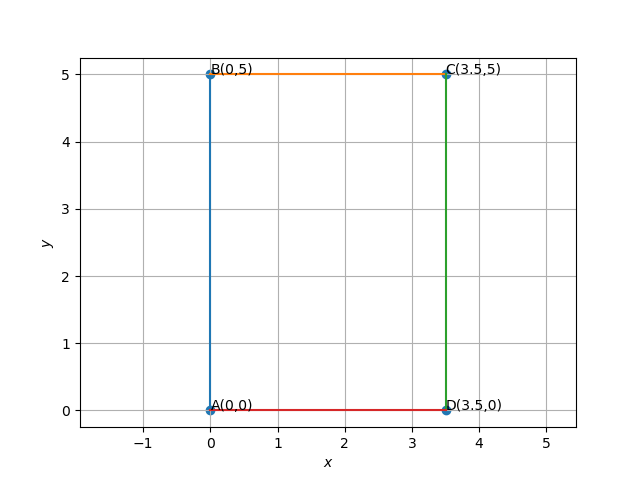
\includegraphics[width = 0.7\columnwidth]{../figs/img.png}
    \caption*{}
    \label{figs}
\end{figure}

\end{document}